\section{Implementation}

\subsection{8-bit DAC Hardware}

A relatively high quality DAC is required in order to synthesize composite
video. AD9748 was selected as it had a fast rise and fall time, parallel input,
and up to 210 MSPS. The only challenge was that no breakout boards existed for
this IC, so a general breakout board was ordered for the QFN-32 package, and
with some help from Ed Casas we managed to reflow solder the IC successfully:

\begin{figure}[H]
    \centering
    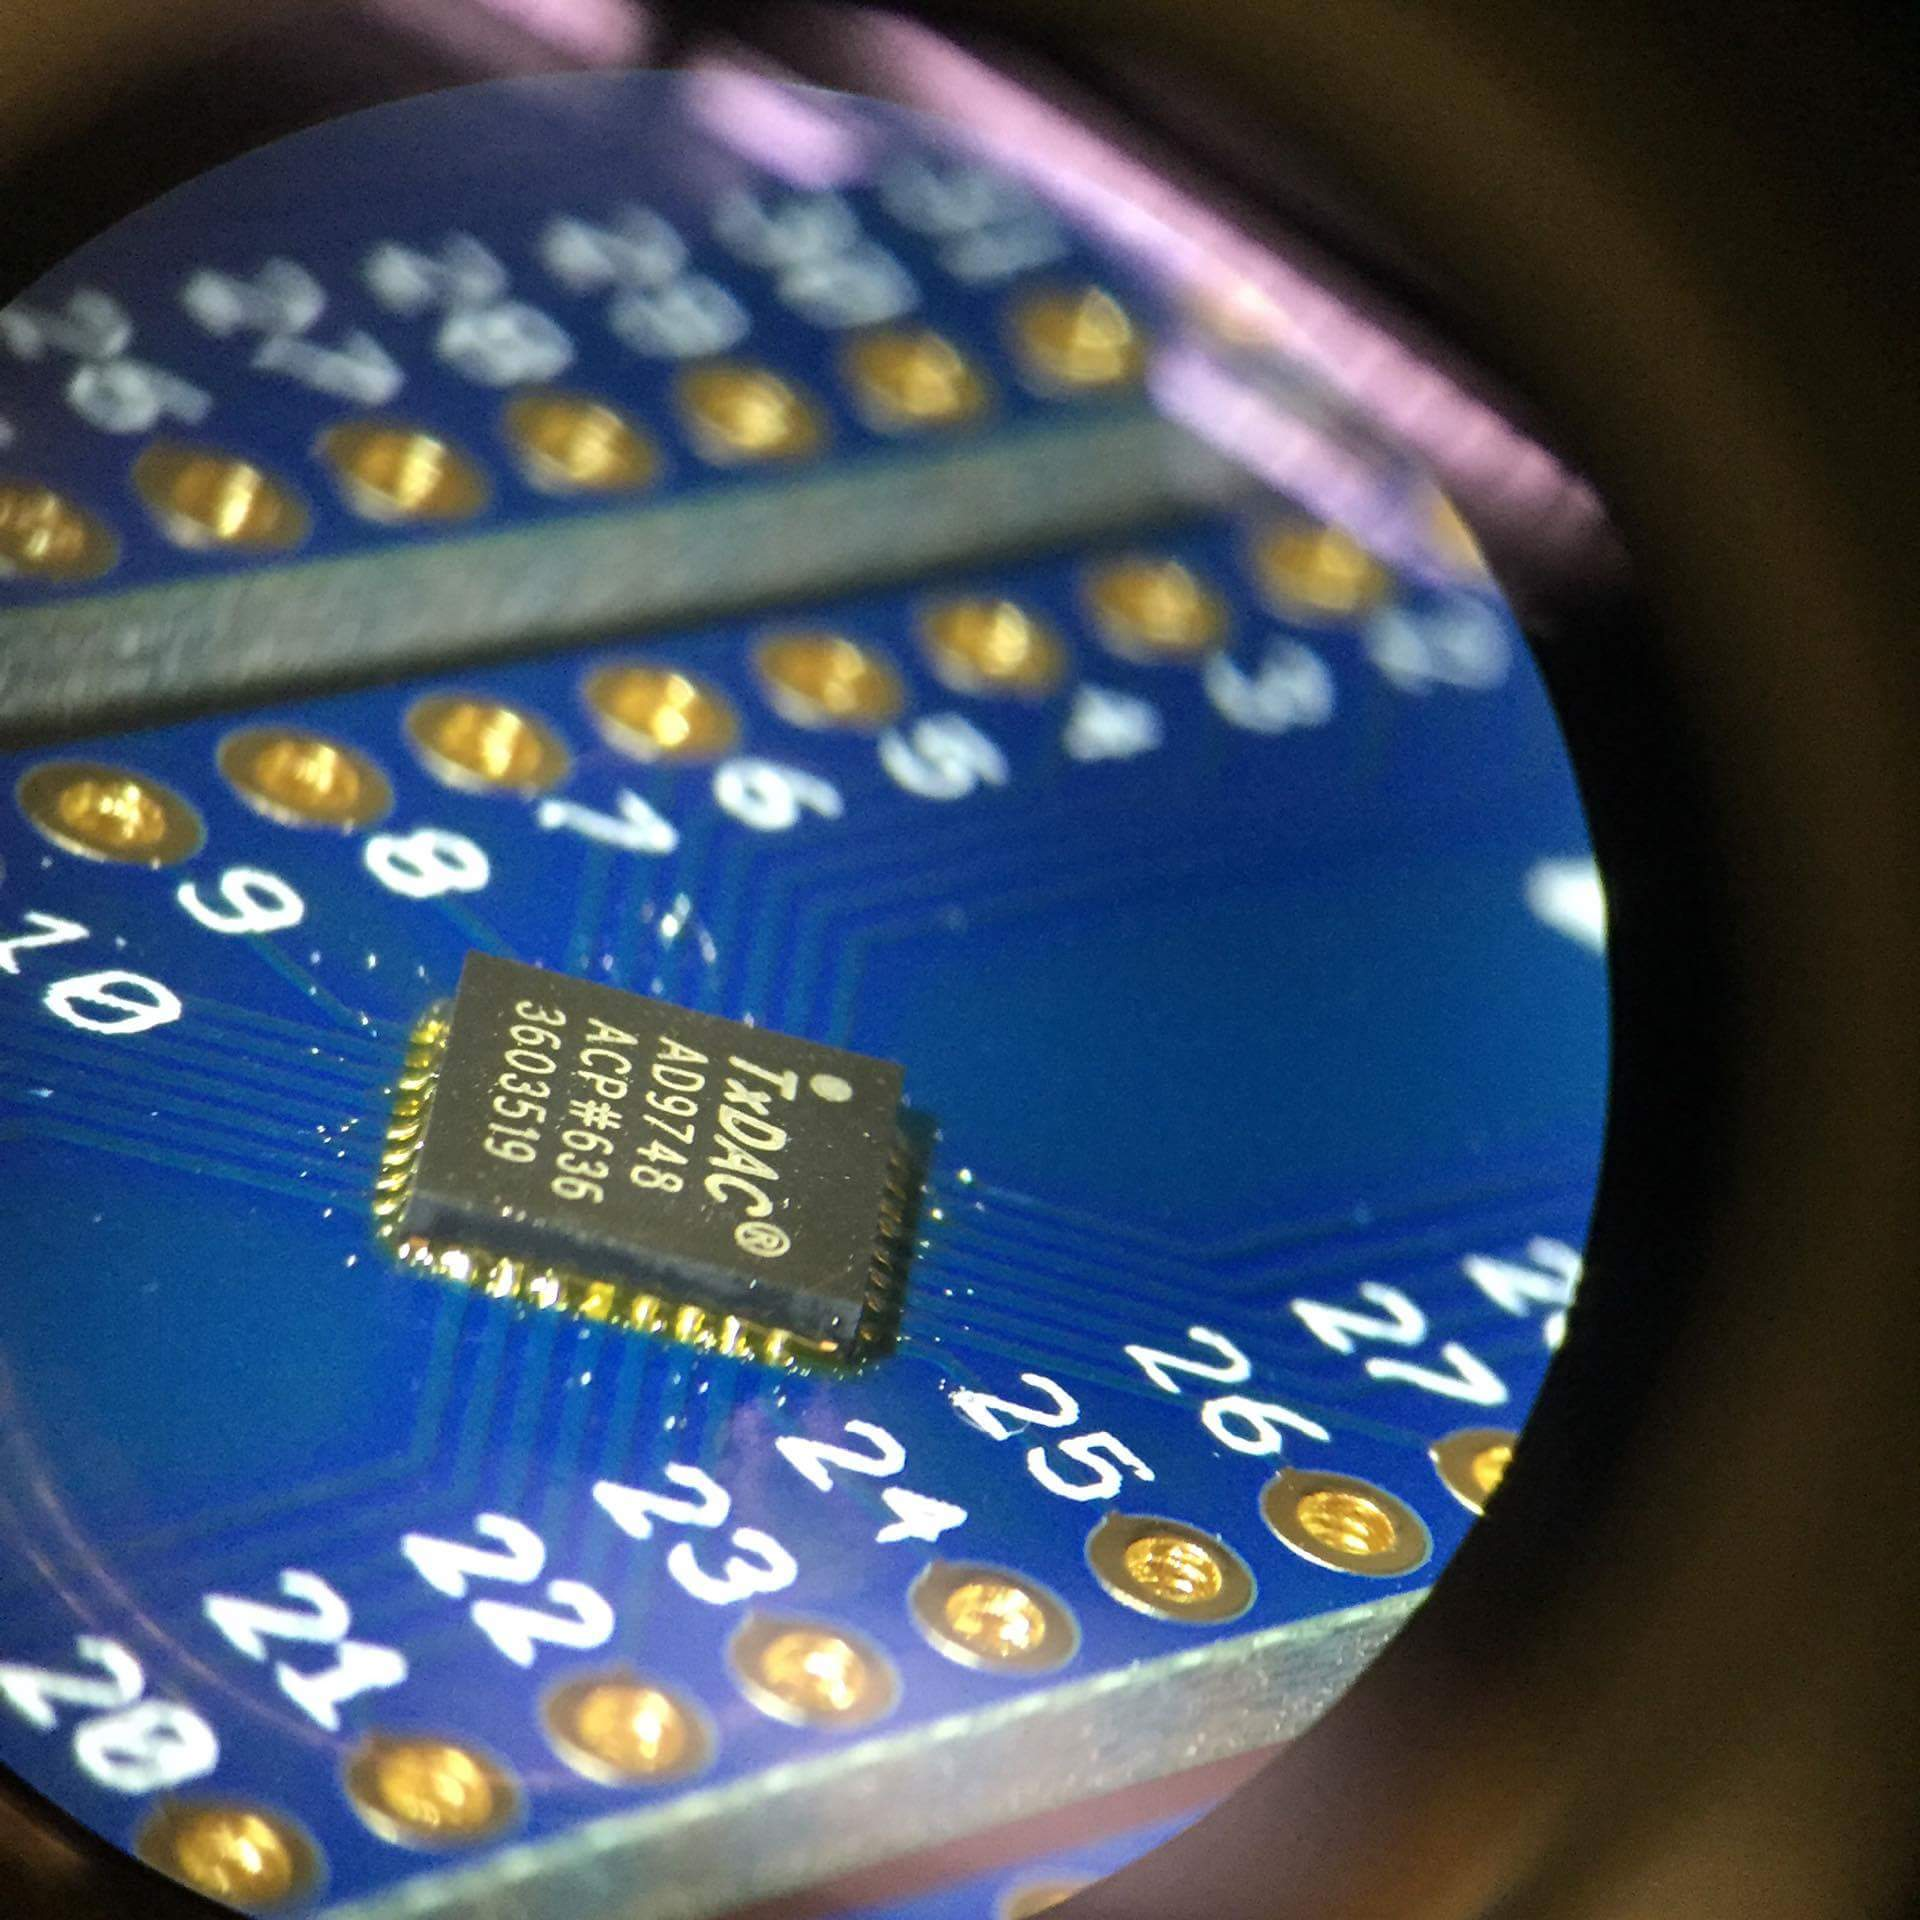
\includegraphics[scale=0.1]{surfaceMount.jpg}
    \caption{Surface Mounted DAC IC}
\end{figure}

As this DAC was going to be operated at 50 MSPS, the clock was put in
differential mode, and a shielded twisted pair was used as the connection
between the FPGA and the DAC board. This was to reduce any possible noise.
additionally the analog power was given a separate regulator that recieved
power from the external dual power supply. The clock and digital power was taken
from the FPGA.

The dual supply is also used to power the video amplifier. This takes the
differential current output of the DAC and converts it into the appropriate
range for composite video (-1V to 1V). The output of the amplifier is connected
to an RCA jack so that it can be easily connected to standard televisions.
Standard value resistors were used for the video amplifier while a potentiometer
was used to adjust the full scale range of the current output of the DAC.

In application we would not be using an external dual power supply but a switching
regulator. This keeps the package size down while only requiring a single power
supply. Additionally the switching power supply would provide some noise
immunity from harmonics created by the 50 MHz clock.

\begin{figure}[H]
    \centering
    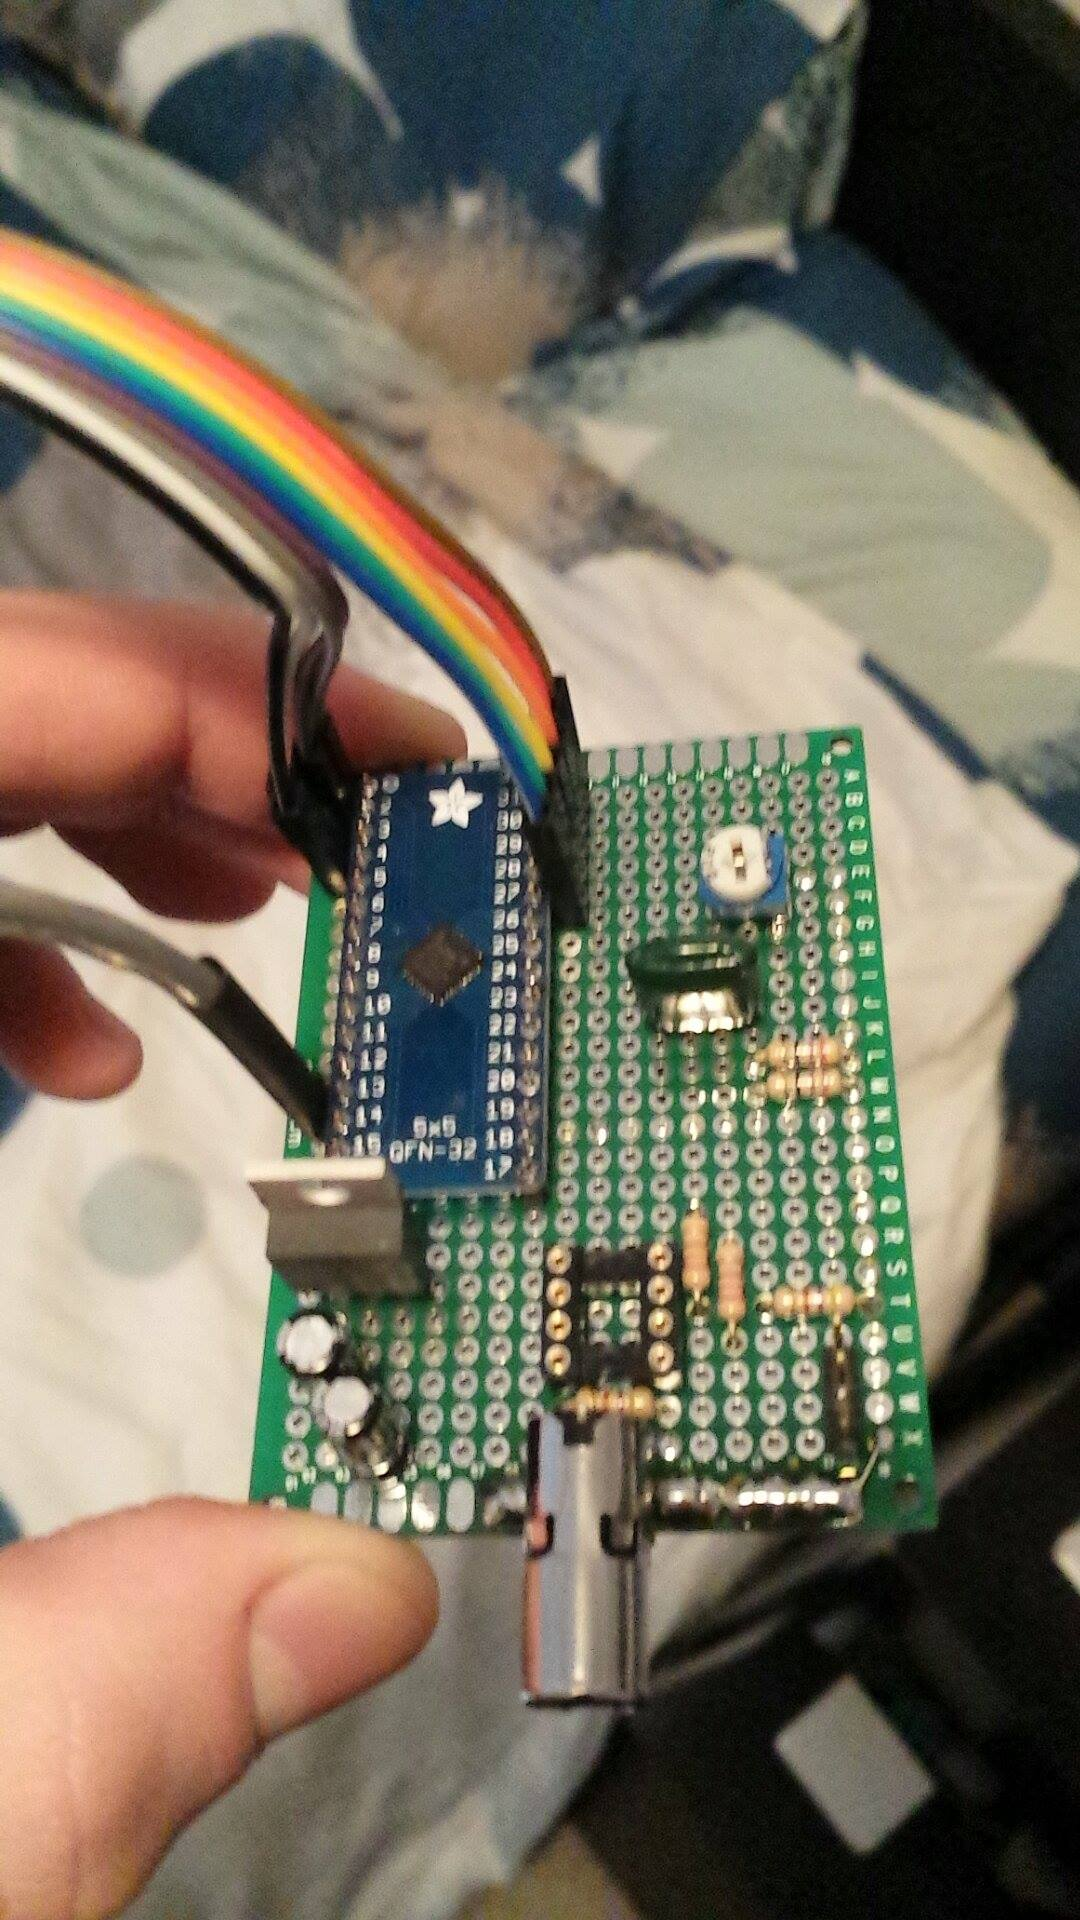
\includegraphics[scale=0.1]{protoBoard.jpg}
    \caption{Prototype DAC Board}
\end{figure}

\subsection{Composite Driver}

\subsubsection{Timing Control}

The challenge with generating composite video is that it is a real-time signal.
Timing of specific synchronizations is important to create an undistorted image.
The timer module controls these timings using a lookup table, a counter, and
some pointers.

Once a vertical blanking signal is needed, the timer is reset to the beginning.
The basic workings of the timer module is that is will have a specific point in
the table, or state. Every clock cycle the counter increments, and once the
counter reaches the value for the next entry in the table, the state increments.
For each entry in the table, there is the count value and the DAC value. 

For the vertical blanking state, the DAC output value will be the Hsync and
Blanking levels which get sent straight to the DAC. When in the horizontal line
state, some of the outputs are Hsync and blanking, however there is the active
video state which switches the DAC output to be driven by the line buffer.
Additional to the clock counter is a pixel counter which increments every 8
clocks so that each pixel in a line is timed perfectly and correct pixel can be
extracted from the line buffer.

\subsubsection{Line Buffer/Block FIFO}

In order to deal with different rates of writing to the DAC and incoming video
data, a buffer that contains all the pixel information for one line was
instantiated in the video generator. A "block" FIFO was used for this buffer.
The idea behind this type of FIFO is that once it is full, it will not accept
any more data until it is reset. Upon a reset, the old data is still available
to the read side until it is overwritten. The video generator would also tell
the SPI module which line it wanted, and so the buffer would get a burst of
writes that would be the line that the video generator was requesting.

\subsubsection{Colour Modulation}

The colour modulation, which did not get to be tested used lookup tables to
decode the colour numbers. A numerically controlled oscillator generated the
phase-time signal for the 3.58 MHz carrier. Phase modulation was done at this
stage since one only needed the addition operator in order to modulate this
signal. Then the phase went into an 8-bit sine lookup table. This was done in
two's compliment so that the dc offset was referenced to the middle of the sine
wave and not the crest. This made generating the lookup tables far simpler. The
sine wave was then amplitude modulated by a value that was assertained from the
colour number using another lookup table. Finally the dc value representing
luminosity was added to the sine wave and the signal was sent to the DAC to be
converted.

\subsection{SPI Module}

The SPI module was designed to take a 9-bit input and a clock input. 8 of the
9 bits was to indicate colour. The last bit was for internal communication. 
Internal communication included setting individual pixels, resetting the frame 
and any other special features the input device could use. Our SPI module was
designed this way so any device, slow or fast, could be used as an input.

Once the SPI module obtained an input, the module would stack two input pixels
and store the input on an array 320 elements long. Each element on the array 
would store 16-bits or two pixels. This make for easy conversion to the SDRAM.
The SDRAM stores 16 bits worth of data at a time.

\subsection{RAM Interface}

The RAM interface was not completed. Although to get this working we would 
needed to use NIOS 2 software to give us a file to be able to access the 
SDRAM. Once this Verilog file would be created we would have to modify it to
fit our needs and properly implement it in our system.

The SDRAM was needed for our project to reach its max potential because the FPGA
could not store enough data alone for a full frame. This is because we needed 
the FPGA to store 640x480 8-bit pixels. At first, we tried to quarter the 
resolution, 320x240, but this still required the use of the SDRAM. When we 
figured we didn’t have enough time to complete the SDRAM module, we lowered the 
resolution again to 160x120. With this resolution, we were finally able to be 
stored an entire frame on the FPGA without using the SDRAM. We stored the data 
on the FPGA in the form if a 160x120 matrix with elements of 8-bit pixels.
